\documentclass[../main/report.tex]{subfiles}
\begin{document}

\chapter{Physical Implementation}
\label{sec:pcb}

\begin{figure}[H]
    \centering
    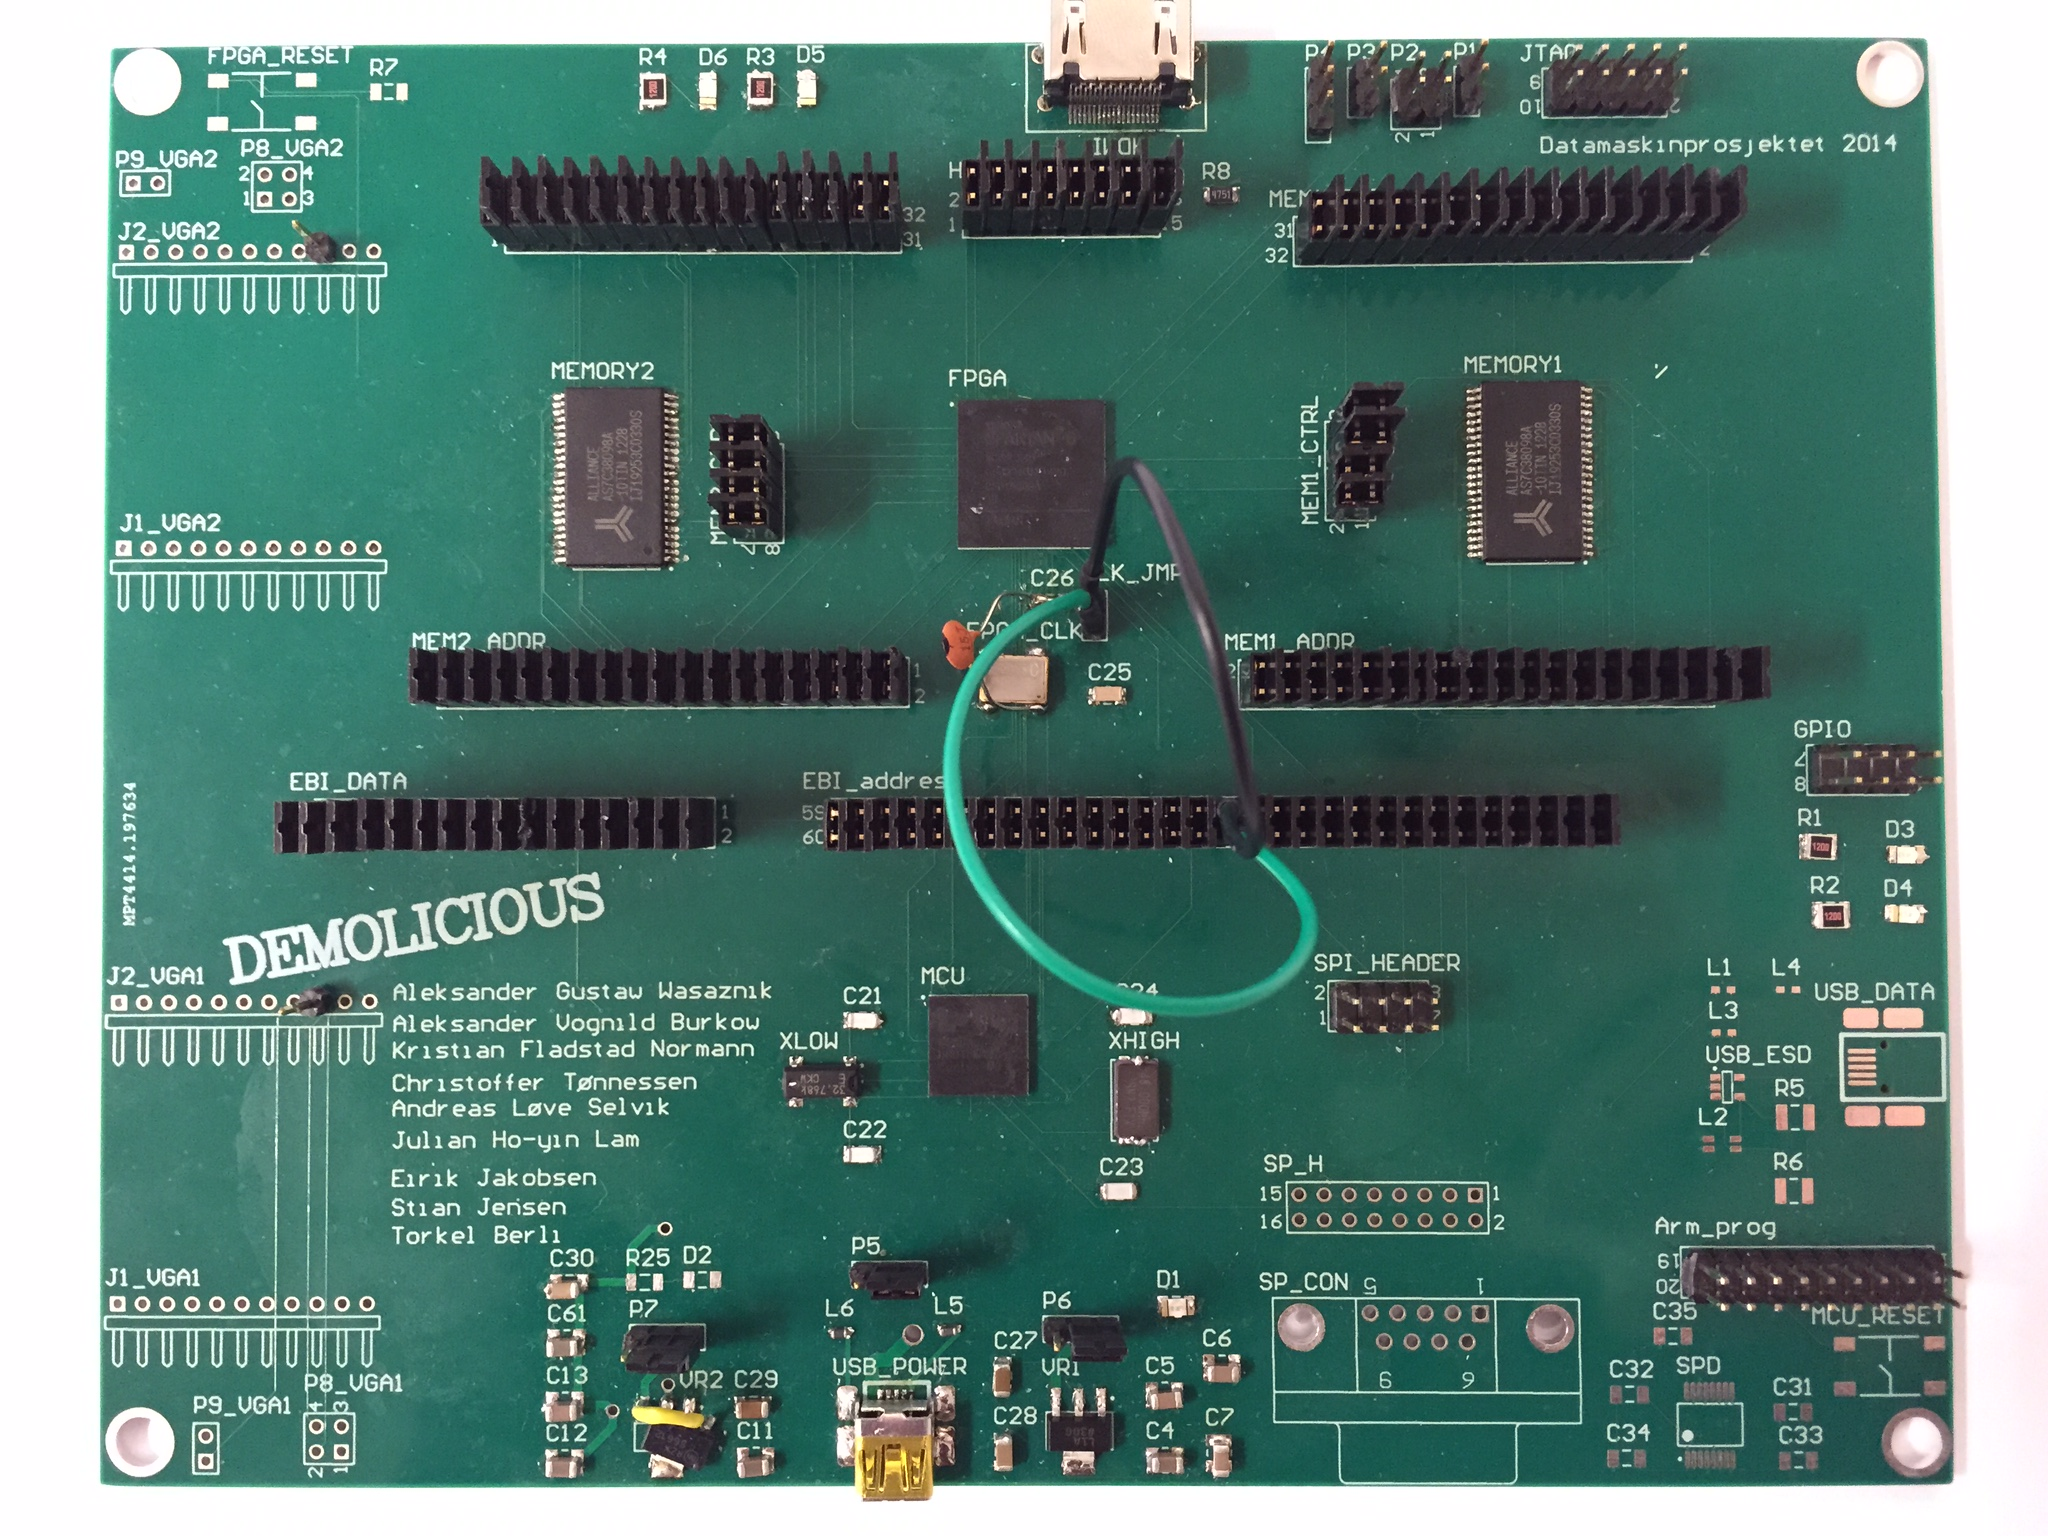
\includegraphics[width=\textwidth]{../pcb/assets/pcb-full.jpg}
    \label{fig:pcb-full}
    \caption{Completed PCB}
\end{figure}

The entire Demolicious system is implemented on a PCB (Printed Circuit Board).
The chapter will give an overview of the hardware architecture
and detail design choices made in the realization of the design.

% Backup oriented design
\subfile{../pcb/backup_oriented_design.tex}

% Input
\subfile{../pcb/input.tex}

% Output
\subfile{../pcb/output.tex}

% Power
\subfile{../pcb/power.tex}

% Bus
\subfile{../pcb/bus.tex}

% Clocks
\subfile{../pcb/clocks.tex}

% Main Components
\subfile{../pcb/components.tex}

\end{document}
